\chapter{\IfLanguageName{dutch}{Proof-of-Concept: Uitvoering en Observaties}{Proof of Concept: Execution and Observations}}
\label{ch:proof_of_concept}

In dit hoofdstuk wordt uitgelegd hoe elk scenario is uitgevoerd in zowel Cisco Packet Tracer als GNS3. Er wordt besproken welke netwerktopologieën zijn gebruikt, welke configuratiestappen belangrijk waren en welke verschillen opvielen tijdens het opzetten en testen. De meetresultaten worden pas uitgebreid besproken in hoofdstuk~5, maar per scenario wordt hier alvast een kort overzicht gegeven van de ervaringen met beide tools. Ter ondersteuning zijn screenshots en figuren toegevoegd. De volledige configuratiebestanden en extra informatie zijn terug te vinden in de bijlagen.

\section{\IfLanguageName{dutch}{Scenario 1 – Point-tot-point verbinding}{Scenario 1 – Point-to-point connection}}
\label{sec:scenario1}

\subsection{\IfLanguageName{dutch}{Topologie}{Topology}}
\label{sec:topologie}

\begin{figure}[H]
    \centering
    \begin{subfigure}[b]{0.48\textwidth}
        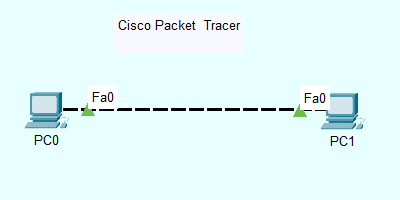
\includegraphics[width=\textwidth]{P2PPacketTracer.png}
        \caption{Point-to-Point in Packet Tracer}
        \label{fig:pt_scenario1}
    \end{subfigure}
    \hfill
    \begin{subfigure}[b]{0.48\textwidth}
        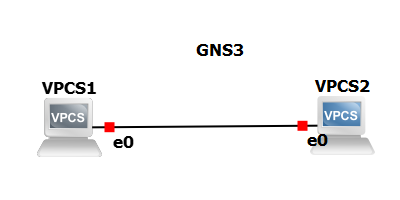
\includegraphics[width=\textwidth]{P2PGNS3.png}
        \caption{Point-to-Point in GNS3}
        \label{fig:gns3_scenario1}
    \end{subfigure}
    \caption[Scenario 1 in beide tools.]{\label{fig:scenario1}Scenario~1 uitgevoerd in zowel Packet Tracer als GNS3.}
\end{figure}



Twee eindapparaten werden rechtstreeks met elkaar verbonden via één UTP-kabel. In \textbf{Packet Tracer} maakten we hiervoor gebruik van twee standaard-pc’s met de namen \texttt{PC0} en \texttt{PC1}. In \textbf{GNS3} stelden we een gelijkaardige situatie voor, maar in plaats van gewone pc’s gebruikten we de \textbf{Virtual PC Simulator (VPCS)}, een lichtgewicht virtuele host die enkel basisnetwerkfunctionaliteit ondersteunt (zoals IP-configuratie, \texttt{ping} en \texttt{traceroute}). VPCS is handig omdat het vrijwel geen resources verbruikt, terwijl het toch toelaat om IP-verkeer te genereren. We noemden ze \texttt{VPCS1} en \texttt{VPCS2}.


\subsection{\IfLanguageName{dutch}{Configuratie in Packet Tracer}{Configuration in Packet Tracer}}
Twee \textbf{pc-iconen} werden op het canvas geplaatst en met elkaar verbonden via een \textbf{Copper Cross-over kabel}. Deze kabel wordt door Packet Tracer doorgaans automatisch geselecteerd bij een verbinding tussen twee pc’s.

Op \texttt{PC0} werd via \texttt{Desktop > IP Configuration} de volgende configuratie ingevoerd:
\begin{itemize}
    \item IP-adres: \texttt{10.0.0.1}
    \item Subnetmasker: \texttt{255.255.255.0}
    \item Gateway: leeg gelaten (niet vereist)
\end{itemize}

Op \texttt{PC1} werd de configuratie als volgt ingesteld:
\begin{itemize}
    \item IP-adres: \texttt{10.0.0.2}
    \item Subnetmasker: \texttt{255.255.255.0}
\end{itemize}

Deze instellingen bleken voldoende. Vervolgens werd op \texttt{PC0}, via het \texttt{Command Prompt} (te vinden onder het tabblad Desktop), het commando \texttt{ping 10.0.0.2} uitgevoerd.

De ping-resultaten waren onmiddellijk positief: de echo-replies keerden terug met \texttt{tijd = 0 ms, TTL = 128}. Hiermee werd de \textbf{connectiviteit succesvol aangetoond}. Verdere configuratie was niet vereist binnen Packet Tracer.

\textit{(Opmerking: Packet Tracer simuleert op de achtergrond automatisch de link-negotiatie en mediadetectie. Dit proces verloopt vrijwel onmiddellijk.)}

\subsection{\IfLanguageName{dutch}{Configuratie in GNS3}{Configuration in GNS3}}

In GNS3 werd gebruikgemaakt van de \textbf{VPCS-functionaliteit} (Virtual PC Simulator). Standaard zijn zes instanties beschikbaar, die via \textit{drag-and-drop} op het canvas geplaatst kunnen worden. Voor dit scenario werden er twee gebruikt.

Een verbinding werd tot stand gebracht tussen \texttt{VPCS1} en \texttt{VPCS2}. In GNS3 wordt dit weergegeven als een eenvoudige lijn, zonder dat een mediumtype hoeft te worden gekozen; de verbinding wordt impliciet als \textbf{ethernetlink} geïnterpreteerd.

Na het starten van de VPCS-nodes (een proces dat slechts een fractie van een seconde in beslag neemt), verschenen voor beide hosts consolevensters. In het console van \texttt{VPCS1} werd het volgende ingevoerd:

\begin{verbatim}
    ip 10.0.0.1/24
\end{verbatim}

Hiermee werd het IP-adres inclusief subnetmasker ingesteld. Omdat beide apparaten zich in hetzelfde subnet bevinden, was geen gateway nodig. In het consolevenster van \texttt{VPCS2} werd ingevoerd:

\begin{verbatim}
    ip 10.0.0.2/24
\end{verbatim}

Vervolgens werd op \texttt{VPCS1} de connectiviteit getest met het commando:

\begin{verbatim}
    ping 10.0.0.2
\end{verbatim}

Vervolgens werd op \texttt{VPCS1} de connectiviteit getest met het commando:

\begin{verbatim}
    ping 10.0.0.2
\end{verbatim}

Alle pingverzoeken kregen een antwoord. De gemeten tijden waren 0.49 ms, 0.92 ms, 0.80 ms, 0.33 ms en 1.63 ms. De eerste reactie kwam onmiddellijk, wat erop wijst dat de ARP-resolutie snel werd uitgevoerd. Er ging geen enkel pakket verloren, en de antwoordtijden waren laag en regelmatig. Dit wijst op een goed werkende point-to-pointverbinding.

De TTL-waarde van 64 geeft aan dat beide hosts zich in hetzelfde subnet bevinden.


\subsection{\IfLanguageName{dutch}{Opmerkingen verschil:}{Opmerkingen verschil:}}
\begin{figure}[H]
    \centering
    \begin{subfigure}[b]{0.48\textwidth}
        \centering
        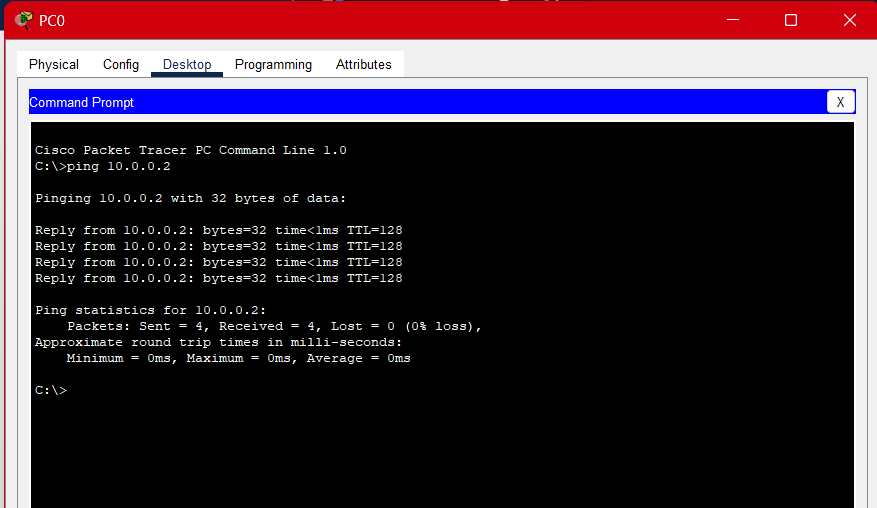
\includegraphics[width=\textwidth]{P2pPacketTracerPing.png}
        \caption{Ping-resultaat in Packet Tracer}
        \label{fig:ping_pt}
    \end{subfigure}
    \hfill
    \begin{subfigure}[b]{0.48\textwidth}
        \centering
        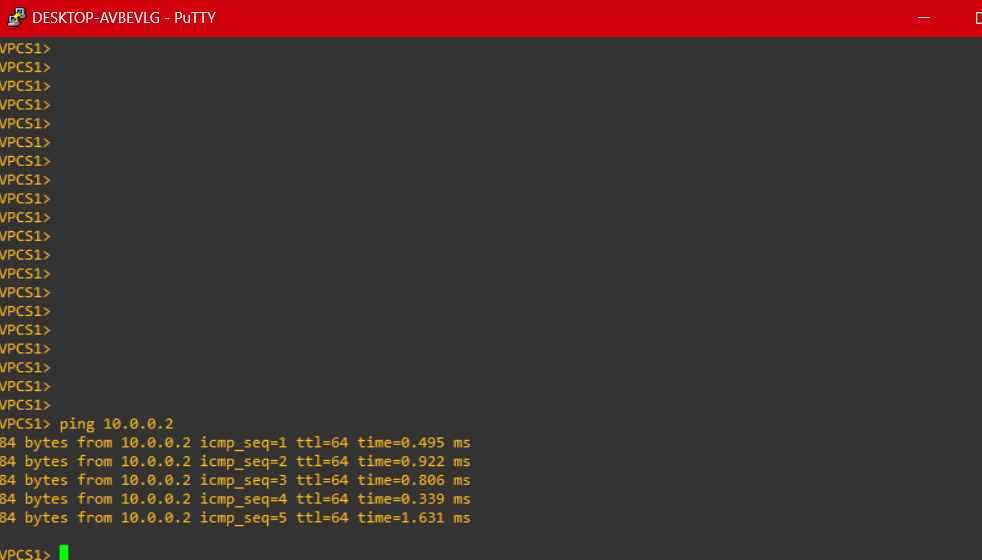
\includegraphics[width=\textwidth]{P2pGNS3Ping.png}
        \caption{Ping-resultaat in GNS3}
        \label{fig:ping_gns3}
    \end{subfigure}
    \caption[Vergelijking van ping-resultaten tussen Packet Tracer en GNS3]{Resultaten van het uitvoeren van een \texttt{ping} tussen twee pc’s in een point-to-point scenario in zowel Packet Tracer als GNS3.}
    \label{fig:ping_pt_gns3}
\end{figure}

Scenario 1 functioneerde correct in zowel \textbf{Packet Tracer} als \textbf{GNS3}. In beide simulatieomgevingen kon een eenvoudige point-to-pointverbinding tussen twee hosts succesvol worden opgezet en getest.

\vspace{0.3cm}

Beide tools leverden uiteindelijk succesvolle netwerkconnectiviteit op, maar tijdens het gebruik kwamen er enkele kleine verschillen naar voren. Packet Tracer maakt vooral gebruik van een grafische interface, waarbij IP-instellingen via vensters en dropdownmenu’s worden ingevoerd. GNS3 daarentegen gebruikt bij VPCS een command line-interface (CLI). Voor absolute beginners kan de grafische benadering in Packet Tracer toegankelijker zijn, terwijl GNS3 meer inzicht biedt in onderliggende netwerkprocessen.

\vspace{0.3cm}

Een opvallend verschil is hoe de pingresultaten worden weergegeven. In Packet Tracer werden alle antwoorden onmiddellijk gegeven, telkens met een gemelde tijd van 0 ms. In GNS3 varieerden de tijden tussen 0.3 en 1.6 ms, wat realistischer is en beter aansluit bij het gedrag van een echt netwerk. Hoewel in dit geval de eerste ping meteen succesvol was, komt de ARP-resolutie normaal gesproken expliciet naar voren. In Packet Tracer blijft dat proces verborgen, tenzij de Simulation Mode wordt ingeschakeld.


\vspace{0.3cm}

De uitvoeringstijd en systeembelasting waren bij beide tools ongeveer gelijk. In zowel Packet Tracer als GNS3 verliep de configuratie vlot, zonder merkbaar tijdsverschil. GNS3’s VPCS gebruikte nauwelijks systeembronnen en had geen meetbare impact op de CPU.

\vspace{0.3cm}

Ook de TTL-waarden verschilden: Packet Tracer gebruikte standaard 128, zoals bij Windows-pc’s. GNS3 past dit aan op het type host; VPCS gedraagt zich als een Linux-systeem en gebruikt daardoor een TTL van 64. Dit maakt de simulatie realistischer. 

\vspace{0.3cm}

Beide tools voldeden aan de vereisten voor dit basisnetwerkscenario. 


\section{\IfLanguageName{dutch}{Scenario 2 – Lokaal netwerk met switch en router}{Scenario 2 – Local Network with Switch and Router}}

\label{sec:scenario2}



\subsection{\IfLanguageName{dutch}{Topologie}{Topology}}
\label{sec:topologie-scenario2}

\begin{figure}[H]
    \centering
    \begin{subfigure}[b]{0.48\textwidth}
        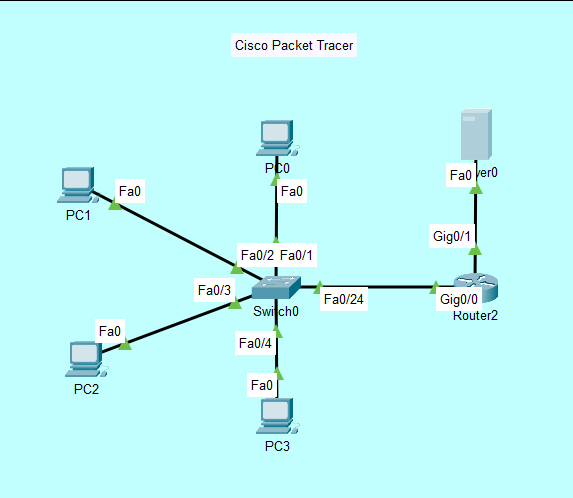
\includegraphics[width=\textwidth]{Sen2PacketTracerTopologie.png}
        \caption{Scenario 2 in Packet Tracer}
        \label{fig:pt_scenario2}
    \end{subfigure}
    \hfill
    \begin{subfigure}[b]{0.48\textwidth}
        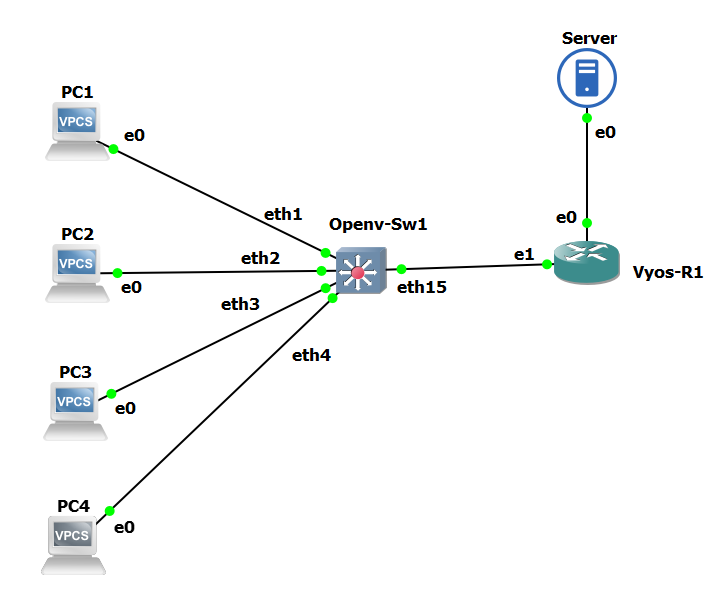
\includegraphics[width=\textwidth]{Sen2GNS3Topologie.png}
        \caption{Scenario 2 in GNS3}
        \label{fig:gns3_scenario2}
    \end{subfigure}
    \caption[Scenario 2 in beide tools.]{\label{fig:scenario2}Scenario~2 uitgevoerd in zowel Packet Tracer als GNS3 met dezelfde netwerkstructuur.}
\end{figure}


In dit scenario stellen we een eenvoudige \textbf{bedrijfsnetwerkomgeving} voor, waarbij meerdere pc’s via een switch zijn verbonden met een router die als gateway fungeert naar een extern netwerk.

\vspace{0.3cm}

Zie Figuur~\ref{fig:scenario2} voor een schematische weergave van de opstelling. In zowel \textbf{Packet Tracer} als \textbf{GNS3} werd dezelfde netwerktopologie opgebouwd: vier pc’s zijn verbonden met één switch, die via een trunkverbinding gekoppeld is aan een router. Op de router zijn subinterfaces geconfigureerd voor twee VLAN’s: \texttt{VLAN10} voor de eerste twee pc’s en \texttt{VLAN20} voor de derde en vierde pc. De router fungeert als gateway voor beide VLAN’s volgens het Router-on-a-Stick-principe.



\vspace{0.3cm}

De buiteninterface van de router is verbonden met een gesimuleerd extern netwerk dat het internet voorstelt, met daarin een server met IP-adres \texttt{8.8.8.8}. De router voert NAT-overload uit om interne clients toegang te geven tot het externe netwerk, en fungeert ook als DHCP-server voor beide VLAN’s. Daarnaast is er een ACL (in Packet Tracer) en een firewall (in GNS3) ingesteld waarbij alleen toestellen in VLAN20 ICMP-verkeer (zoals pings) mogen sturen naar de externe server. Verkeer vanuit VLAN10 wordt daarbij geblokkeerd. Deze opstelling biedt de mogelijkheid om het gedrag van netwerktoegang en verkeersfiltering in verschillende situaties  te observeren en te vergelijken. 


In \textbf{GNS3} werd dezelfde topologie opgebouwd als in Packet Tracer, maar met open-source componenten zoals \texttt{VyOS} en \texttt{Open vSwitch}, aangezien officiële Cisco IOS-images enkel via een licentie verkregen kunnen worden.


\textbf{Extra componenten:}
\begin{itemize}
    \item De router fungeert als DHCP-server en wijst automatisch IP-adressen toe aan de pc’s in beide VLAN’s.
    \item NAT-overload is geconfigureerd zodat interne pc’s toegang krijgen tot het externe netwerk via één publiek IP-adres.
    \item Een ACL in \textbf{Packet Tracer} en een firewall in \textbf{GNS3} bepaalt dat enkel bepaalde hosts (zoals in VLAN20) ICMP-verkeer naar een specifieke externe server mogen sturen, terwijl ander ICMP-verkeer wordt geblokkeerd.
\end{itemize}

\vspace{0.5cm}

\subsubsection{\IfLanguageName{dutch}{Configuratie in Packet Tracer}{Configuration in Packet Tracer}}

In \textbf{Packet Tracer} werden vier pc’s toegevoegd, samen met één switch (type \texttt{2960}) en een \texttt{2911}-router. PC0 en PC1 zijn verbonden met VLAN10, PC2 en PC3 met VLAN20. Daarnaast werd een server toegevoegd aan de buiteninterface van de router om het externe netwerk te simuleren. Deze server kreeg het IP-adres \texttt{8.8.8.8}.

\textbf{1. Switchconfiguratie (Cisco 2960):}
\begin{verbatim}
    enable
    configure terminal
    
    vlan 10
    name Client10
    exit
    
    vlan 20
    name Client20
    exit
    
    vlan 100
    name Trunk
    exit
    
    interface range fa0/1 - 2
    switchport mode access
    switchport access vlan 10
    exit
    
    interface range fa0/3 - 4
    switchport mode access
    switchport access vlan 20
    exit
    
    interface fa0/24
    switchport mode trunk
    switchport trunk native vlan 100
    end
    
    
\end{verbatim}

\textbf{2. Routerconfiguratie (Cisco 2811):}

\begin{verbatim}
    interface g0/0.10
    encapsulation dot1Q 10
    ip address 192.168.10.254 255.255.255.0
    ip nat inside
    ip access-group 101 in
    exit
    
    interface g0/0.20
    encapsulation dot1Q 20
    ip address 192.168.20.254 255.255.255.0
    ip nat inside
    ip access-group 101 in
    exit
\end{verbatim}

\textbf{Stap 2: Hoofdinterface activeren}

\begin{verbatim}
    interface g0/0
    no shutdown
    exit
\end{verbatim}

\textbf{Stap 3: WAN-interface (naar internet) configureren}

\begin{verbatim}
    interface g0/1
    ip address 8.8.8.1 255.255.255.0
    ip nat outside
    ip access-group 101 in
    no shutdown
    exit
\end{verbatim}

\textbf{Stap 4: DHCP-configuratie}

De router krijgt twee DHCP-pools mee, één per VLAN. Elke pool deelt IP-adressen uit binnen het subnet van het respectieve VLAN.

\begin{verbatim}
    ip dhcp pool NET10
    network 192.168.10.0 255.255.255.0
    default-router 192.168.10.254
    dns-server 8.8.8.8
    exit
    
    ip dhcp pool NET20
    network 192.168.20.0 255.255.255.0
    default-router 192.168.20.254
    dns-server 8.8.8.8
    exit
\end{verbatim}

\textbf{Stap 5: NAT-configuratie}

Hier wordt NAT overload ingesteld zodat alle interne hosts via \texttt{G0/1} toegang tot internet kunnen krijgen.

\begin{verbatim}
    access-list 1 permit 192.168.0.0 0.0.255.255
    ip nat inside source list 1 interface g0/1 overload
\end{verbatim}

\textbf{Stap 6: Access Control List (ACL)}

ACL 101 zorgt ervoor dat alleen VLAN 20 (192.168.20.0/24) toegang heeft tot de server \texttt{8.8.8.8}. VLAN 10 wordt geblokkeerd. Alle ander verkeer wordt toegestaan.

\begin{verbatim}
    access-list 101 permit ip 192.168.20.0 0.0.0.255 host 8.8.8.8
    access-list 101 deny ip 192.168.10.0 0.0.0.255 host 8.8.8.8
    access-list 101 permit ip any any
\end{verbatim}


\subsubsection{\IfLanguageName{dutch}{Configuratie in GNS3}{Configuration in GNS3}}

In \textbf{GNS3} werd dezelfde topologie opgebouwd als in Packet Tracer. Vier \texttt{VPCS}-hosts zijn via \texttt{Open vSwitch} verbonden met een \texttt{VyOS}-router. PC1 en PC2 behoren tot \texttt{VLAN10}, PC3 en PC4 tot \texttt{VLAN20}. De trunkverbinding loopt van poort \texttt{eth15} op de switch naar \texttt{eth1} op de router. De WAN-verbinding verloopt via \texttt{eth0} naar een externe server (\texttt{8.8.8.8}). 

De structuur en werking zijn identiek aan de Packet Tracer-topologie, maar worden hier gerealiseerd met open-source tools.


\textbf{1. Switchconfiguratie (Open vSwitch):}
\begin{verbatim}
    # VLAN 10 - Access
    ovs-vsctl set port eth1 tag=10
    ovs-vsctl set port eth2 tag=10
    
    # VLAN 20 - Access
    ovs-vsctl set port eth3 tag=20
    ovs-vsctl set port eth4 tag=20
    
    # Trunk naar VyOS-router
    ovs-vsctl set port eth15 trunks=10,20
\end{verbatim}

\textbf{2. Routerconfiguratie (VyOS):}
\begin{verbatim}
    configure
    
    # WAN-interface (naar internet)
    set interfaces ethernet eth0 address '8.8.8.1/24'
    
    # Subinterfaces voor VLAN 10 en 20 op eth1
    set interfaces ethernet eth1 vif 10 address '192.168.10.254/24'
    set interfaces ethernet eth1 vif 20 address '192.168.20.254/24'
\end{verbatim}

\textbf{Stap 2: NAT-configuratie}
\begin{verbatim}
    set nat source rule 100 description 'NAT voor LAN naar WAN'
    set nat source rule 100 source address '192.168.0.0/16'
    set nat source rule 100 outbound-interface name eth0
    set nat source rule 100 translation address masquerade
\end{verbatim}

\textbf{Stap 3: DHCP-configuratie}
\begin{verbatim}
    # VLAN 10
    set service dhcp-server shared-network-name VLAN10 subnet 192.168.10.0/24 subnet-id 1
    set service dhcp-server shared-network-name VLAN10 subnet 192.168.10.0/24 range 0 start '192.168.10.10'
    set service dhcp-server shared-network-name VLAN10 subnet 192.168.10.0/24 range 0 stop '192.168.10.100'
    set service dhcp-server shared-network-name VLAN10 subnet 192.168.10.0/24 range 0 option default-router '192.168.10.254'
    set service dhcp-server shared-network-name VLAN10 subnet 192.168.10.0/24 range 0 option name-server '8.8.8.8'
    
    # VLAN 20
    set service dhcp-server shared-network-name VLAN20 subnet 192.168.20.0/24 subnet-id 2
    set service dhcp-server shared-network-name VLAN20 subnet 192.168.20.0/24 range 0 start '192.168.20.10'
    set service dhcp-server shared-network-name VLAN20 subnet 192.168.20.0/24 range 0 stop '192.168.20.100'
    set service dhcp-server shared-network-name VLAN20 subnet 192.168.20.0/24 range 0 option default-router '192.168.20.254'
    set service dhcp-server shared-network-name VLAN20 subnet 192.168.20.0/24 range 0 option name-server '8.8.8.8'
\end{verbatim}

\textbf{Stap 4: Firewallconfiguratie (ter vervanging van ACL)}
\begin{verbatim}
    set firewall ipv4 name VLAN-ACCESS rule 10 action 'accept'
    set firewall ipv4 name VLAN-ACCESS rule 10 source address '192.168.20.0/24'
    set firewall ipv4 name VLAN-ACCESS rule 10 destination address '8.8.8.8'
    
    set firewall ipv4 name VLAN-ACCESS rule 20 action 'drop'
    set firewall ipv4 name VLAN-ACCESS rule 20 source address '192.168.10.0/24'
    set firewall ipv4 name VLAN-ACCESS rule 20 destination address '8.8.8.8'
    
    set firewall ipv4 name VLAN-ACCESS rule 30 action 'accept'
\end{verbatim}

\textbf{Stap 5: Zones definiëren}
\begin{verbatim}
    set firewall zone LAN default-action drop
    set firewall zone LAN member interface eth1.10
    set firewall zone LAN member interface eth1.20
    
    set firewall zone WAN default-action drop
    set firewall zone WAN member interface eth0
    
    set firewall zone WAN from LAN firewall name VLAN-ACCESS
    set firewall zone WAN from LAN default-action drop
    
    commit
    save
\end{verbatim}


\subsection{\IfLanguageName{dutch}{Opmerkingen verschil:}{Opmerkingen verschil:}}

In scenario 2 werden de verschillen tussen beide tools al snel duidelijk. In GNS3 kan men niet onmiddellijk beginnen met het opbouwen van een topologie. Eerst moeten geschikte VyOS- en Open vSwitch-images worden gedownload en gekoppeld aan de GNS3-VM. Pas daarna kunnen de netwerkcomponenten worden toegevoegd en geconfigureerd. Hoewel dit met een duidelijke handleiding goed uitvoerbaar is, vraagt het meer technische voorbereiding, inzicht en extra tijd dan bij Cisco Packet Tracer. In Packet Tracer zijn de Cisco-router en -switch direct beschikbaar, waardoor het integreren van pc’s, switches en routers snel en zonder bijkomende configuratie verloopt.

\vspace{0.3cm}

Ook op het vlak van systeemprestaties zijn er verschillen merkbaar. Het opstarten van virtuele apparaten in GNS3 vraagt meer rekenkracht. De VyOS-router en Open vSwitch veroorzaken een tijdelijke piek in het CPU-gebruik, die na het volledig opstarten weer terugvalt naar een stabiel niveau. Packet Tracer werkt met interne simulatie waarbij apparaten onmiddellijk beschikbaar zijn en de belasting van het systeem minimaal blijft. Dit maakt Packet Tracer bijzonder efficiënt voor eenvoudige netwerkscenario’s. GNS3 biedt daarentegen realistischer netwerkgedrag. Alles start iets trager op, maar ik had wel meer controle en kon makkelijker zien waar iets fout liep.

\vspace{0.3cm}

Wat betreft de tijdsbesteding viel op dat het configuratieproces in GNS3 duidelijk meer tijd vroeg dan in Cisco Packet Tracer. Voor scenario 2 kon het volledige netwerk in Packet Tracer binnen 15 minuten worden opgebouwd en getest. In GNS3 liep de benodigde tijd op tot 30 tot 35 minuten. Deze extra tijd was vooral het gevolg van het opstarten van de virtuele componenten: zowel de VyOS-router als Open vSwitch moesten volledig actief zijn voordat de configuratie kon beginnen. Voor de rest waren de configuratiestappen en het eindresultaat identiek in beide omgevingen. Dezelfde configuratie kon zonder aanpassingen worden toegepast in zowel Packet Tracer als GNS3, met vergelijkbare werking.

\vspace{0.3cm}

\begin{figure}[H]
    \centering
    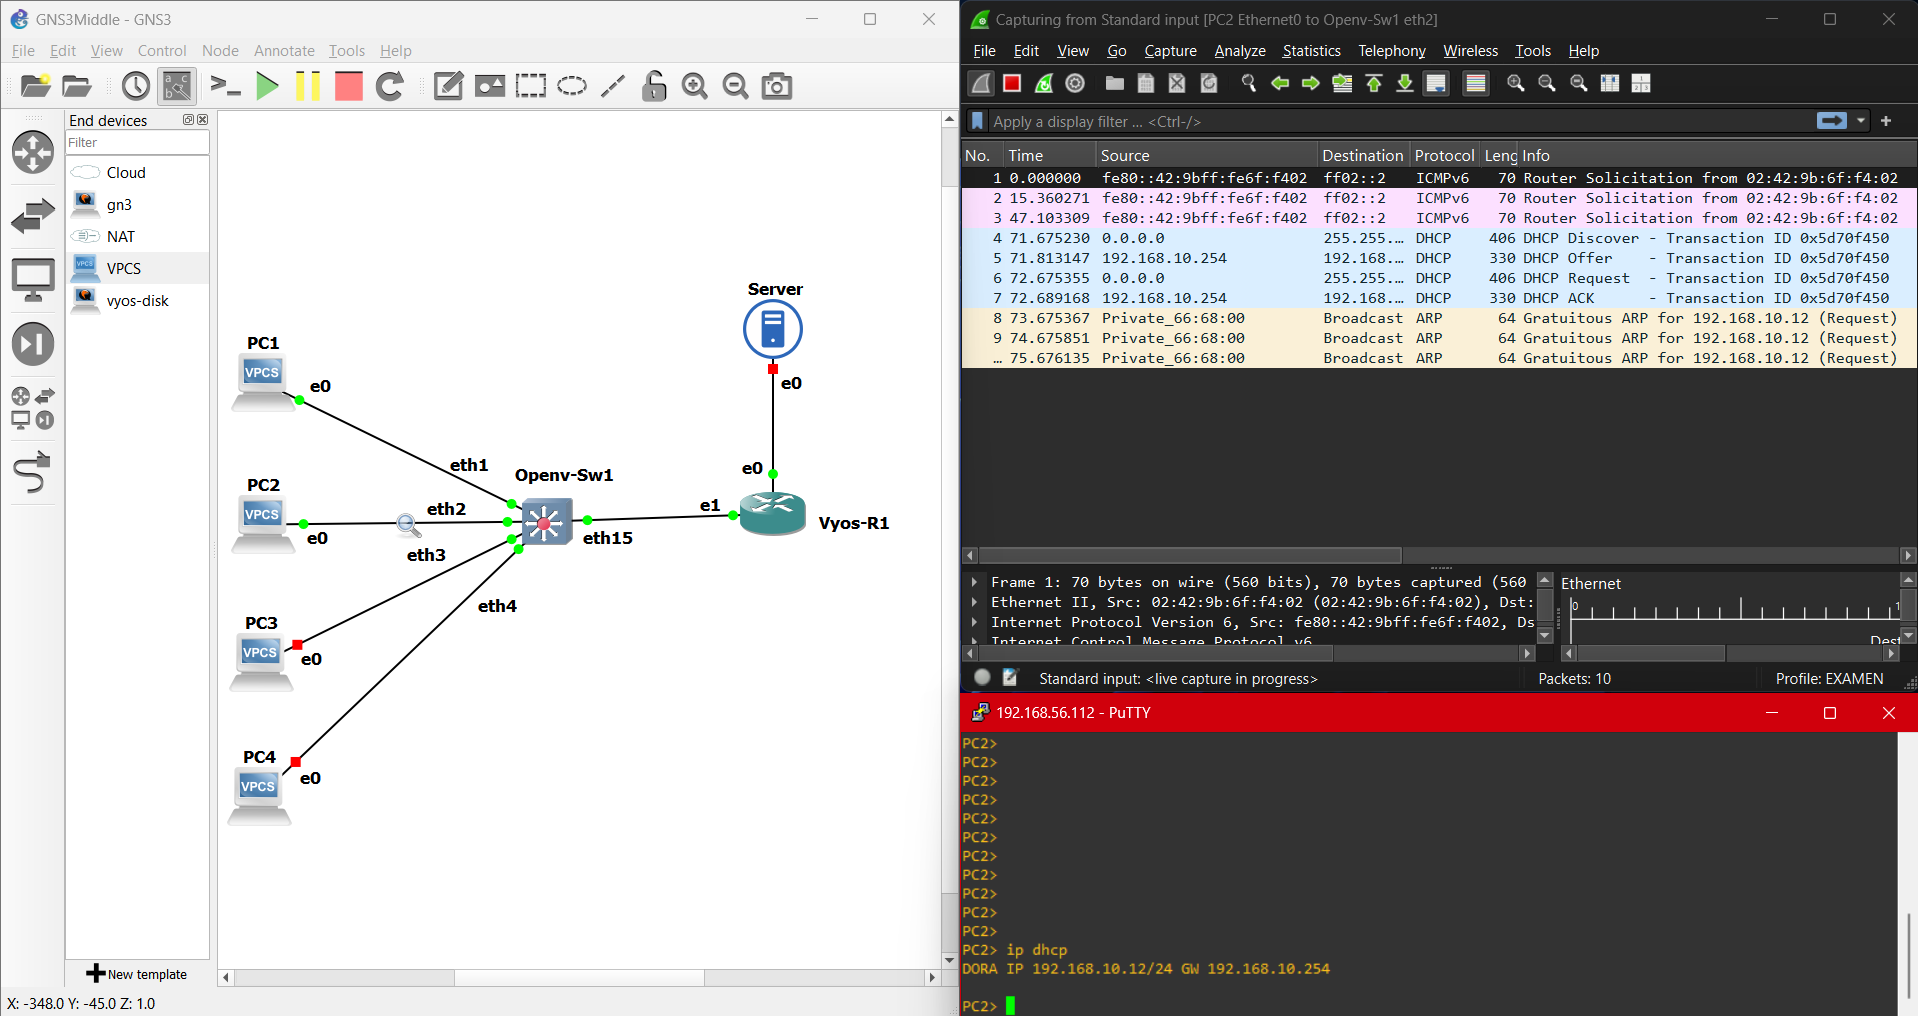
\includegraphics[width=0.7\textwidth]{WeergaveDHCPGns3.png}
    \caption{DHCP-proces zichtbaar in GNS3 via packet capture.}
    \label{fig:dhcp_gns3}
\end{figure}


Een bijkomend voordeel van werken in GNS3 is dat het mogelijk maakt om netwerkverkeer tot in detail te observeren. Zoals weergegeven in afbeelding ~\ref{fig:dhcp_gns3} , verschijnen na het opstarten van de router automatisch verschillende netwerkberichten in de packet capture. PC2 stuurt eerst een verzoek uit om een router in het netwerk te vinden. Kort daarna start het volledige DHCP-proces. De computer vraagt een IP-adres aan en ontvangt vervolgens een geldig adres samen met de standaardgateway. Dit bevestigt dat de DHCP-configuratie correct is uitgevoerd.

\vspace{0.3cm}

\begin{figure}[H]
    \centering
    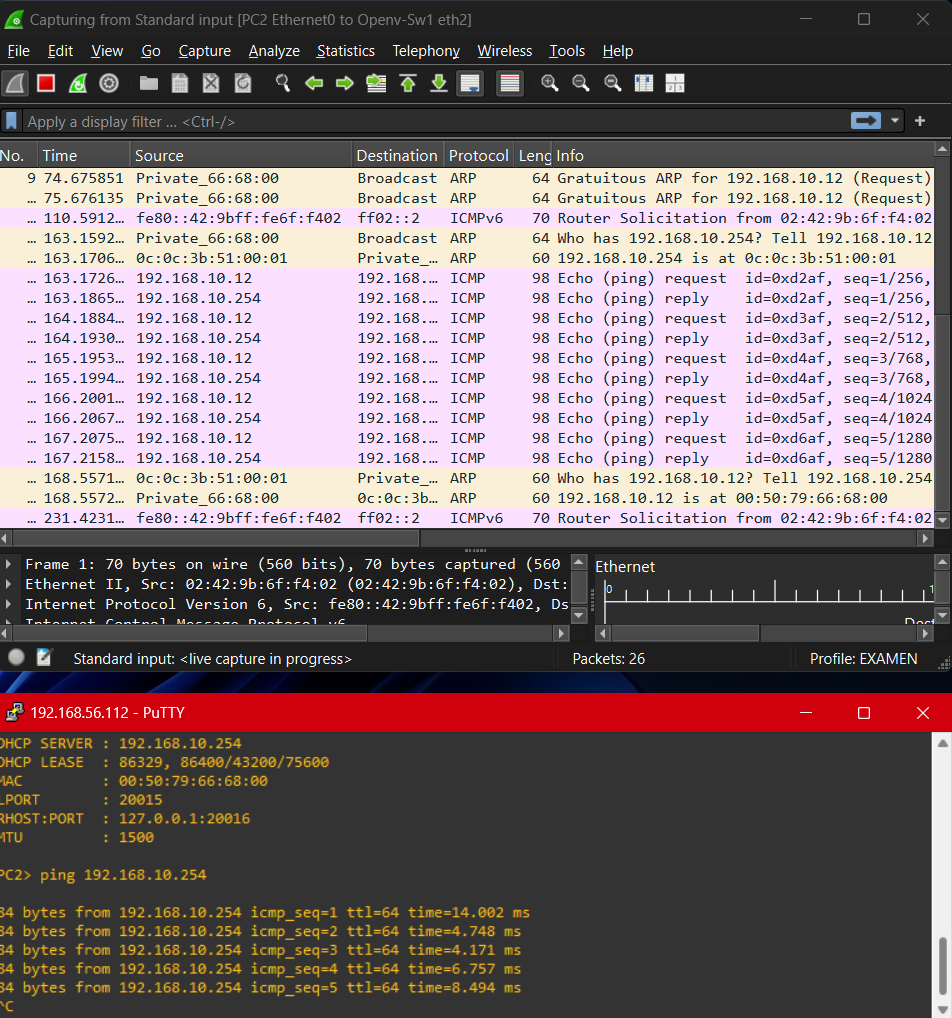
\includegraphics[width=0.7\textwidth]{PingverkeerTussenPCEnRouter.png}
    \caption{Pingverkeer tussen PC2 en de router in GNS3.}
    \label{fig:ping_gns3}
\end{figure}

In afbeelding ~\ref{fig:ping_gns3} wordt dit verder getest met een ping naar het adres van de router. Daarbij zijn zowel het pingbericht als het antwoord zichtbaar, samen met de tijd die nodig is om te reageren. Deze manier van testen benadert sterk de werking van een echt netwerk.

\vspace{0.3cm}

In Cisco Packet Tracer verloopt dit proces op basis van vooraf gesimuleerde processen. De configuratie werkt functioneel, maar de communicatie tussen apparaten wordt niet zichtbaar gemaakt. De DHCP-aanvraag gebeurt automatisch op de achtergrond, zonder dat de tussenliggende stappen of datapakketten weergegeven worden. Ook bij een ping zie je enkel het eindresultaat, zonder details over het verloop. Hierdoor is het moeilijker om fouten op te sporen of inzicht te krijgen in hoe het netwerk reageert. GNS3 biedt in dat opzicht meer transparantie en realisme, en is daardoor beter geschikt om netwerkprocessen grondig te analyseren.






\section{\IfLanguageName{dutch}{Scenario 3 – Complex netwerk (CCNA-Niveau 3)}{Scenario 3 – Complex netwerk (CCNA-Niveau 3}}
\label{sec:scenario3}

\subsection{\IfLanguageName{dutch}{Topologie Scenario 3}{Topology Scenario 3}}
\label{sec:topologie-scenario3}

\begin{figure}[H]
    \centering
    \begin{subfigure}[b]{0.48\textwidth}
        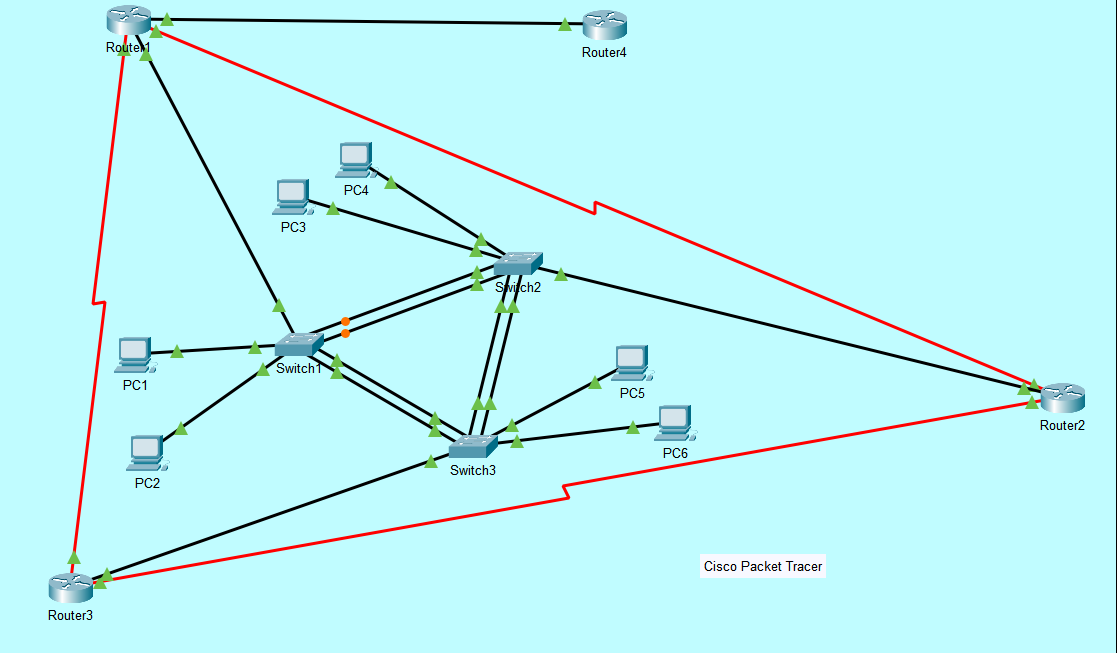
\includegraphics[width=\textwidth]{Sen3PacketTracerTopologie.png}
        \caption{Scenario 3 in Packet Tracer}
        \label{fig:pt_scenario3}
    \end{subfigure}
    \hfill
    \begin{subfigure}[b]{0.48\textwidth}
        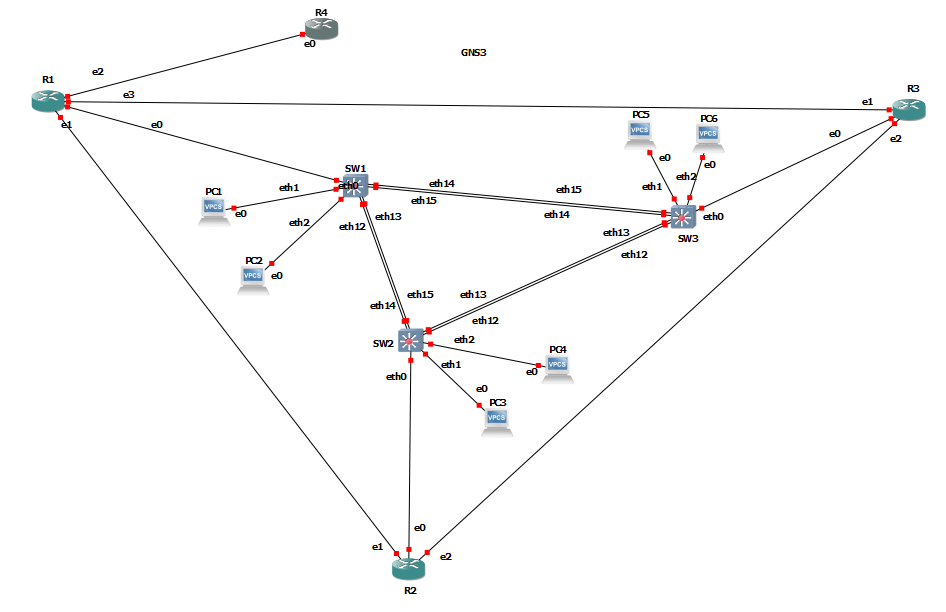
\includegraphics[width=\textwidth]{Sen3Gns3Topologie.png}
        \caption{Scenario 3 in GNS3}
        \label{fig:gns3_scenario3}
    \end{subfigure}
    \caption[Scenario 3 in beide tools.]{\label{fig:scenario3}Scenario~3 uitgevoerd in zowel Packet Tracer als GNS3 met vergelijkbare netwerkstructuur.}
\end{figure}



In dit scenario bouwen we een uitgebreid netwerk dat drie afzonderlijke locaties met elkaar verbindt. De structuur van deze opstelling wordt weergegeven in Figuur~\ref{fig:scenario3}.

\vspace{0.3cm}

Elke locatie beschikt over een eigen router (R1, R2 en R3) en een eigen switch (SW1, SW2 en SW3). De routers zijn verbonden volgens een driehoekstopologie, waardoor er steeds meerdere paden beschikbaar zijn tussen de verschillende sites. Deze topologie is opgezet om de werking van OSPF-routing binnen een redundante netwerkstructuur te demonstreren.

\vspace{0.3cm}

Elke switch is geconfigureerd met twee VLAN’s: VLAN10 en VLAN20. In elk VLAN bevindt zich één pc, zodat elke locatie logisch is opgesplitst in aparte afdelingen of gebruikersgroepen.

\vspace{0.3cm}

Router R1 is verbonden met een vierde router (R4) die als internetgateway fungeert. Om internettoegang mogelijk te maken, vertaalt R1 de interne IP-adressen naar een publiek IP-adres via NAT-overload.

\vspace{0.3cm}

Op alle drie de routers is OSPF ingesteld voor dynamische routering. De IP-adrestoewijzing gebeurt via twee DHCP-servers: R2 beheert VLAN10 en R3 verzorgt VLAN20.


\vspace{0.3cm}

Elke switch is gekoppeld aan zijn router en ook rechtstreeks verbonden met de andere switches via trunklinks en EtherChannels. Door deze opstelling ontstaat een driehoek op laag 2. STP, dat standaard actief is, voorkomt automatisch netwerkloops door één van de verbindingen te blokkeren.


\subsubsection{\IfLanguageName{dutch}{Configuratie in Packet Tracer}{Configuration in Packet Tracer}}
\label{sec:configuratie-PacketTracer}

De volgende configuratie werd toegepast op de routers en switches in Scenario~2. Aangezien veel instellingen gelijkaardig zijn, zijn de configuratieblokken gegroepeerd per toesteltype.

\vspace{0.3cm}

\paragraph{Router R1: Gateway + NAT + DHCP + OSPF}
\begin{verbatim}
    interface g0/0.10
    encapsulation dot1Q 10
    ip address 10.1.10.254 255.255.255.0
    ip nat inside
    ip access-group 101 in
    exit
    
    interface g0/0.20
    encapsulation dot1Q 20
    ip address 10.1.20.254 255.255.255.0
    ip nat inside
    ip access-group 101 in
    exit
    
    interface g0/0
    no shutdown
    exit
    
    interface g0/1
    ip address 192.0.2.1 255.255.255.0
    ip nat outside
    no shutdown
    exit
    
    interface s0/3/0
    ip address 10.10.12.1 255.255.255.252
    clock rate 64000
    ip nat inside
    no shutdown
    exit
    
    interface s0/3/1
    ip address 10.10.13.1 255.255.255.252
    ip nat inside
    no shutdown
    exit
    
    ip dhcp excluded-address 10.1.10.1 10.1.10.99
    ip dhcp excluded-address 10.1.20.1 10.1.20.99
    
    access-list 1 permit 10.0.0.0 0.255.255.255
    ip nat inside source list 1 interface g0/1 overload
    
    ip route 0.0.0.0 0.0.0.0 192.0.2.254
    
    router ospf 1
    network 10.0.0.0 0.255.255.255 area 0
    network 10.10.12.0 0.0.0.3 area 0
    network 10.10.13.0 0.0.0.3 area 0
    network 192.0.2.0 0.0.0.255 area 0
    default-information originate
\end{verbatim}

\vspace{0.3cm}
\paragraph{Routers R2 en R3 (gelijkend, met aangepaste IP's)}
(Sterk gelijkaardig aan R1, maar met eigen subnetten)
\textit{Voorbeeld R2:}
\begin{verbatim}
    interface g0/0.10
    encapsulation dot1Q 10
    ip address 10.2.10.254 255.255.255.0
    ip nat inside
    exit
    
    interface s0/3/0
    ip address 10.10.12.2 255.255.255.252
    ip nat inside
    no shutdown
    exit
    
    ip dhcp pool VLAN10
    network 10.2.10.0 255.255.255.0
    default-router 10.2.10.254
    dns-server 8.8.8.8
    
    router ospf 1
    network 10.10.12.0 0.0.0.3 area 0
\end{verbatim}

\vspace{0.3cm}

\paragraph{Router R4: Internet-router}
\begin{verbatim}
    interface g0/0
    ip address 192.0.2.254 255.255.255.0
    no shutdown
    exit
    ip route 0.0.0.0 0.0.0.0 GigabitEthernet0/0
    
    ip route 0.0.0.0 0.0.0.0 g0/0
\end{verbatim}

\vspace{0.3cm}
\paragraph{Switch SW1–SW3: VLAN-configuratie + Trunk + EtherChannel}
(SW1 voorbeeld)
\begin{verbatim}
    vlan 10
    name Client10
    vlan 20
    name Client20
    
    interface fa0/2
    switchport mode access
    switchport access vlan 10
    exit
    interface fa0/3
    switchport mode access
    switchport access vlan 20
    exit
    
    interface fa0/1
    switchport mode trunk
    switchport trunk allowed vlan 10,20
    exit
    
    interface range fa0/23 - 24
    switchport mode trunk
    channel-group 1 mode desirable
    exit
    
    interface Port-channel1
    switchport mode trunk
    switchport trunk allowed vlan 10,20
    exit
\end{verbatim}



\subsubsection{\IfLanguageName{dutch}{Configuratie in GNS3}{Configuration in GNS3}}
\label{sec:configuratie-Gns3}

\subsubsection{\IfLanguageName{dutch}{Configuratie in GNS3}{Configuration in GNS3}}
\label{sec:configuratie-GNS3}

In GNS3 werd hetzelfde netwerk nagebouwd met \textbf{VyOS-routers} en \textbf{Open vSwitch (OVS)}-switches. De configuratie wordt hieronder per toesteltype weergegeven, waarbij gelijkaardige instellingen gegroepeerd zijn om herhaling te vermijden.

\vspace{0.3cm}
\paragraph{Router R1: Gateway + NAT + DHCP + OSPF}
\begin{verbatim}
    configure
    
    set interfaces ethernet eth0 vif 10 address '10.1.10.254/24'
    set interfaces ethernet eth0 vif 10 description 'VLAN10'
    set interfaces ethernet eth0 vif 20 address '10.1.20.254/24'
    set interfaces ethernet eth0 vif 20 description 'VLAN20'
    set interfaces ethernet eth0 description 'Trunk to Switch'
    set interfaces ethernet eth1 address '192.0.2.1/24'
    set interfaces ethernet eth1 description 'Internet'
    set interfaces ethernet eth2 address '10.10.12.1/30'
    set interfaces ethernet eth3 address '10.10.13.1/30'
    
    set nat source rule 10 source address '10.0.0.0/8'
    set nat source rule 10 outbound-interface 'eth1'
    set nat source rule 10 translation address 'masquerade'
    
    set protocols static route 0.0.0.0/0 next-hop 192.0.2.254
    
    set protocols ospf area 0 network 10.0.0.0/8
    set protocols ospf parameters router-id 1.1.1.1
    set protocols ospf redistribute static
    
    commit
    save
\end{verbatim}

\vspace{0.3cm}
\paragraph{Router R2: DHCP + OSPF}
\begin{verbatim}
    configure
    
    set interfaces ethernet eth0 vif 10 address '10.2.10.254/24'
    set interfaces ethernet eth0 vif 20 address '10.2.20.254/24'
    set interfaces ethernet eth0 description 'Trunk'
    set interfaces ethernet eth1 address '10.10.12.2/30'
    set interfaces ethernet eth2 address '10.10.23.1/30'
    
    set service dhcp-server shared-network-name VLAN10 subnet 10.2.10.0/24 \
    default-router '10.2.10.254' dns-server '8.8.8.8' range 0 start '10.2.10.100' stop '10.2.10.200'
    
    set protocols ospf area 0 network 10.0.0.0/8
    set protocols ospf parameters router-id 2.2.2.2
    
    commit
    save
\end{verbatim}

\vspace{0.3cm}
\paragraph{Router R3: DHCP + OSPF}
\begin{verbatim}
    configure
    
    set interfaces ethernet eth0 vif 10 address '10.3.10.254/24'
    set interfaces ethernet eth0 vif 20 address '10.3.20.254/24'
    set interfaces ethernet eth0 description 'Trunk'
    set interfaces ethernet eth1 address '10.10.23.2/30'
    set interfaces ethernet eth2 address '10.10.13.2/30'
    
    set service dhcp-server shared-network-name VLAN20 subnet 10.3.20.0/24 \
    default-router '10.3.20.254' dns-server '8.8.8.8' range 0 start '10.3.20.100' stop '10.3.20.200'
    
    set protocols ospf area 0 network 10.0.0.0/8
    set protocols ospf parameters router-id 3.3.3.3
    
    commit
    save
\end{verbatim}

\vspace{0.3cm}

\paragraph{Router R4: Internet + Statische route}
\begin{verbatim}
    configure
    
    set interfaces ethernet eth0 address '192.0.2.254/24'
    set protocols static route 0.0.0.0/0 next-hop '192.0.2.1'
    
    commit
    save
\end{verbatim}

\vspace{0.3cm}
\paragraph{Switches SW1–SW3: Open vSwitch configuratie (OVS)}
\textit{Voorbeeld voor SW1}
\begin{verbatim}
    # Access ports voor PC1 en PC2
    ovs-vsctl set port eth1 tag=10
    ovs-vsctl set port eth2 tag=20
    
    # Trunk naar Router1
    ovs-vsctl set port eth0 trunks=10,20
    
    # EtherChannel bond1 (naar SW2 via eth12 + eth13)
    ovs-vsctl add-bond br0 bond1 eth12 eth13
    ovs-vsctl set port bond1 trunks=10,20
    
    # EtherChannel bond2 (naar SW3 via eth14 + eth15)
    ovs-vsctl add-bond br0 bond2 eth14 eth15
    ovs-vsctl set port bond2 trunks=10,20
\end{verbatim}

\subsection{\IfLanguageName{dutch}{Opmerkingen verschil:}{Opmerkingen verschil:}}

Scenario 3 was de meest uitgebreide test in deze vergelijking. Het netwerk was opgebouwd uit meerdere routers en switches, waarbij verschillende protocollen werden toegepast. Naast de functionele werking werd ook gekeken naar configuratietijd en systeemprestaties. Daardoor kwamen de verschillen tussen Cisco Packet Tracer en GNS3 duidelijk naar voren.

\vspace{0.3cm}

Tijdens de uitvoering bleek er een significant verschil in de benodigde tijd en systeembelasting tussen beide platforms. In Cisco Packet Tracer kon het volledige netwerk binnen ongeveer 40 minuten worden opgebouwd en getest. De apparaten waren meteen beschikbaar en reageerden vrijwel onmiddellijk, waardoor de configuratie vlot verliep. In GNS3 daarentegen duurde het opzetten van hetzelfde netwerk ongeveer 1 uur en 20 minuten. Deze langere opstarttijd werd, net als in Scenario 2, vooral veroorzaakt door het laden van de virtuele toestellen. De VyOS-router bijvoorbeeld heeft enkele minuten nodig om volledig op te starten, en ook andere componenten moeten eerst actief zijn vooraleer er kon worden gestart met configureren en testen. Dit zorgde voor een merkbare vertraging in de beginfase van het configuratieproces.

\vspace{0.3cm}



Ook op het vlak van systeembelasting waren de verschillen duidelijk. Tijdens het opstarten van GNS3 steeg het CPU-gebruik tijdelijk tot 100\%. Zodra alle apparaten actief waren, stabiliseerde het verbruik tussen 47\% en 69\%, afhankelijk van de netwerkactiviteit0\. In tegenstelling daarmee bleef het CPU-gebruik in Packet Tracer doorgaans onder de 20\%. Dit verschil is logisch, aangezien GNS3 gebruikmaakt van echte virtuele machines, terwijl Packet Tracer werkt met gesimuleerde apparaten in een geoptimaliseerde omgeving(zie figuur~\ref{fig:cpu_verbruik}).

\vspace{0.3cm}

\begin{figure}[H]
    \centering
    \begin{subfigure}[b]{0.48\textwidth}
        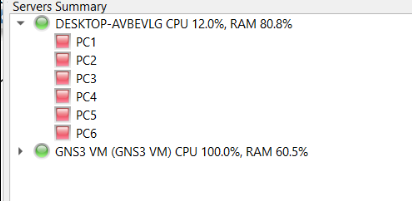
\includegraphics[width=\textwidth]{CpuVerbruik1.png}
        \caption{CPU-gebruik tijdens het opstarten van GNS3}
        \label{fig:cpu_opstart}
    \end{subfigure}
    \hfill
    \begin{subfigure}[b]{0.48\textwidth}
        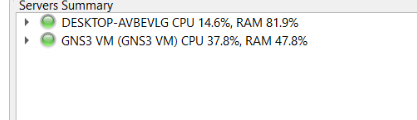
\includegraphics[width=\textwidth]{CpuVerbruik2.png}
        \caption{Gestabiliseerd CPU-gebruik na opstart}
        \label{fig:cpu_na_opstart}
    \end{subfigure}
    \caption[CPU-verbruik van GNS3 tijdens Scenario 3.]{\label{fig:cpu_gns3}CPU-verbruik van GNS3 bij het opstarten en na stabilisatie tijdens Scenario~3.}
\end{figure}


Een bijkomend voordeel van GNS3 is de mogelijkheid om het volledige OSPF-proces te analyseren via Wireshark. Tijdens een packet capture zijn alle fasen van het protocol zichtbaar, zoals Hello-pakketten, Database Description, Link State Request, Link State Update en Link State Acknowledgement. Dit biedt een gedetailleerd inzicht in het verloop van het routingproces. In Packet Tracer zijn deze stappen niet waarneembaar; daar zijn enkel visuele statusindicatoren beschikbaar, wat de analyse beperkt.(zie figuur~\ref{fig:ospf_wireshark}).

\begin{figure}[H]
    \centering
    
    \begin{subfigure}[b]{\textwidth}
        \centering
        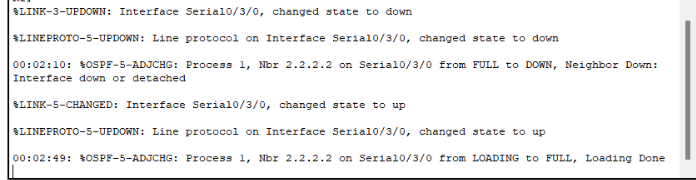
\includegraphics[width=\textwidth]{OSPFBerichten1.png}
        \caption{Packet Tracer: OSPF-berichten op Router 1}
        \label{fig:ospf_r1}
    \end{subfigure}
    
    \vspace{1em}
    
    \begin{subfigure}[b]{\textwidth}
        \centering
        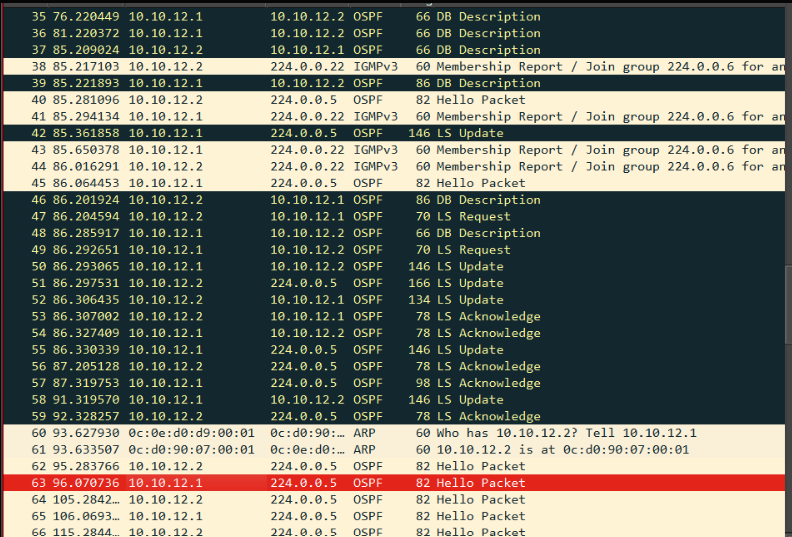
\includegraphics[width=\textwidth]{OSPFBerichten2.png}
        \caption{Wireshark: OSPF-berichten op Router 2}
        \label{fig:ospf_r2}
    \end{subfigure}
    
    \vspace{1em}
    
    \begin{subfigure}[b]{\textwidth}
        \centering
        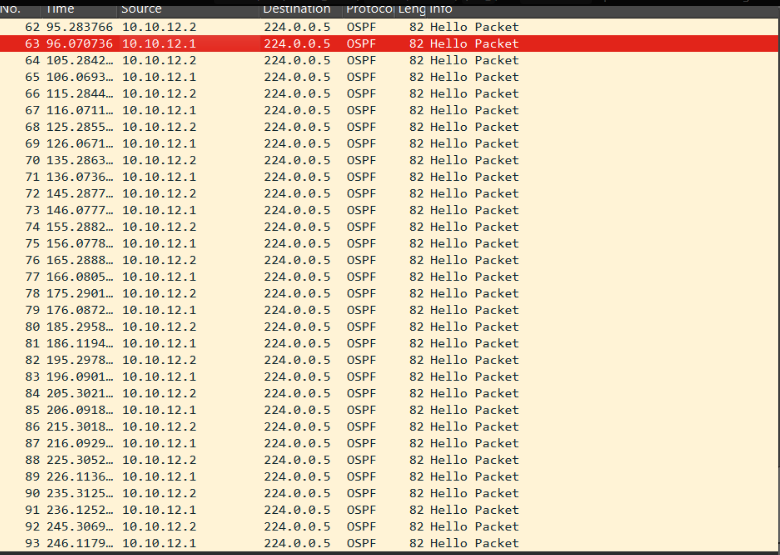
\includegraphics[width=\textwidth]{OSPFBerichten3.png}
        \caption{Wireshark: OSPF-berichten op Router 3}
        \label{fig:ospf_r3}
    \end{subfigure}
    
    \caption[OSPF-verkeer zichtbaar via Wireshark in GNS3.]{\label{fig:ospf_wireshark}Weergave van het OSPF-proces via Wireshark in GNS3 op drie verschillende routers. In Packet Tracer zijn deze details niet zichtbaar.}
\end{figure}



\vspace{0.3cm}

Die mogelijkheid maakt het niet alleen eenvoudiger om netwerkinfrastructuren te testen, maar ook om verschillende vakgebieden te integreren. Binnen één scenario kunnen studenten werken rond besturingssystemen, serverbeheer, virtualisatie en netwerkbeheer. Ze kunnen hun configuraties in GNS3 eerst volledig uittesten in een virtuele omgeving en die vervolgens toepassen op echte apparatuur. Dit zorgt ervoor dat de overstap van oefening naar praktijk veel vlotter, realistischer en efficiënter verloopt.

\vspace{0.3cm}

Voor Scenario 3 werd er bewust gekozen om de opstelling eenvoudig te houden en goed vergelijkbaar te maken met Cisco Packet Tracer. Hoewel het technisch mogelijk was om in GNS3 een volledige Linux-host te gebruiken, is daar bewust niet voor gekozen. Om een eerlijke vergelijking te kunnen maken, werd gewerkt met een standaard VPCS, die qua functionaliteit beter aansluit bij de gesimuleerde pc’s in Packet Tracer. De focus lag op basisfunctionaliteiten zoals routingprotocollen, configuratietijd en gebruiksvriendelijkheid, zodat de verschillen tussen beide platformen op een duidelijke en evenwichtige manier konden worden vastgesteld.

